\chapter{Conclusion}

\section {Future Work}

\subsection {Training}

The author believes that the accuracy of RideSafes detection algorithm could greatly be improved with more comprehensive training data. Due to time constraints the data used for training the machine learning model is not as diverse as intended. The training data used for ride safe during tested was collected only from two riders. As discussed throughout even with the most common types of crashes displaying similar patterns, no two riders are identical.   With RideSafe performing as it does one can only deduce performance would improve with a more generalized model to begin with eventually leading to a more personalized model over time.





\subsection {Collaboration}

Currently on the market popular ride tracking applications severely lack  any safeguards for the users safety, popular cycling oriented fitness tracking applications such as Trailforks or Strava actively monitor the users speed and location. Without major redesigns for either party the crash detection logic present in RideSafe could be implemented as a supplementary feature for the benefit of the users. Since the most power intensive feature of RideSafe is GPS functionality, the algorithm could be added to Strava or Trailforks adding only marginally higher power consumption then they already have.




\subsection {Inter-Device communication}
RideSafe would greatly benefit with a companion server. Three major improvements could be made with server-device communication 


\subsection *{Communal Accident HeatMap}

Crash locations collected from all users around the world could be collected to populate a global heatmap accessible to all users. All accident sites from all users could produce an accurate depiction of where danger may be present, potentially saving users from riding dangerous trails or locations. The map could easily be split into an all time accident heatmap as well as showing only recent accidents which could indicate a trail which recently became hazardous, such as a fallen tree or a dislodged rock.



\subsection *{Push Notifications}
Once a crash is detected fellow local users of RideSafe could be sent a distress notification. By locating the nearest users, a distress call could be put out. As the emergency services can take quite a while to arrive, perhaps a local first aider cold reach the scene in advance.




\subsection *{Shared Training Data}
Crash data collected from all users automatically pushed to a server could be used to create a shared dataset of training data, benefiting all users and improving RideSafes generalized model.



\subsection *{Performance Improvements}


As suggested to the author external speedometers for bicycles are readily available and inexpensive. As GPS is currently used to calculate speed in Ridesafe improvements in terms of battery performance and accuracy can be made by using an external speedometer. These Bluetooth enabled devices communicating using ANT+ can be fitted to any bicycle to calculate speed and if utilized device battery life would greatly improve. 

\newpage
\section {Conclusion}

 The purpose of this project was to develop a simple to use crash detection application using machine learning in real-time, and by doing so potentially save someone's life. As shown from the results, this goal was achieved. The author is delighted to have been able to achieve all aims originally set in the planning stage of RideSafe, as well as achieving all the personal goals set in chapter 1. RideSafe may not be ready for a full release at time of writing but the author was adamant to make their presence on the google play store, as shown in figure \ref{store} RideSafe is currently available for open beta testing. Working in an area where specific relevant sensor data is not publically available has been a challenging experience, discovering unknowns, alone has been a very rewarding experience to which the author is extremely proud to have achieved. To the best of the authors knowledge RideSafe is the first sensor based application to use speed as a factor in determining whether a crash has occurred as well as classifying live sensor readings in real-time on a single device.

All functional requirements have been accomplished as well as laying down the foundations for many non-functional requirements. With time constraints as well as the logistics involved with real world testing and training, development of RideSafe has not been an easy feat to complete, however it has been a truly rewarding experience. Choosing to undertake my own idea for a project was daunting at first, with so many unknown variables at play at the beginning I had my doubts at the feasibility of completing this project. My motivation to create an application which one day may save a life kept me focused to reach my end goal. 

 By researching the innovations made in the medical domain as well analysing the pitfalls of existing solutions, the development of RideSafe has shown that existing solutions may not always be the optimal solution. 


%%%%%%%%%%%%%%%%%%%%%%%%%%%%%%%%%%%%%%%%
\begin{figure}[h]
      \centering
      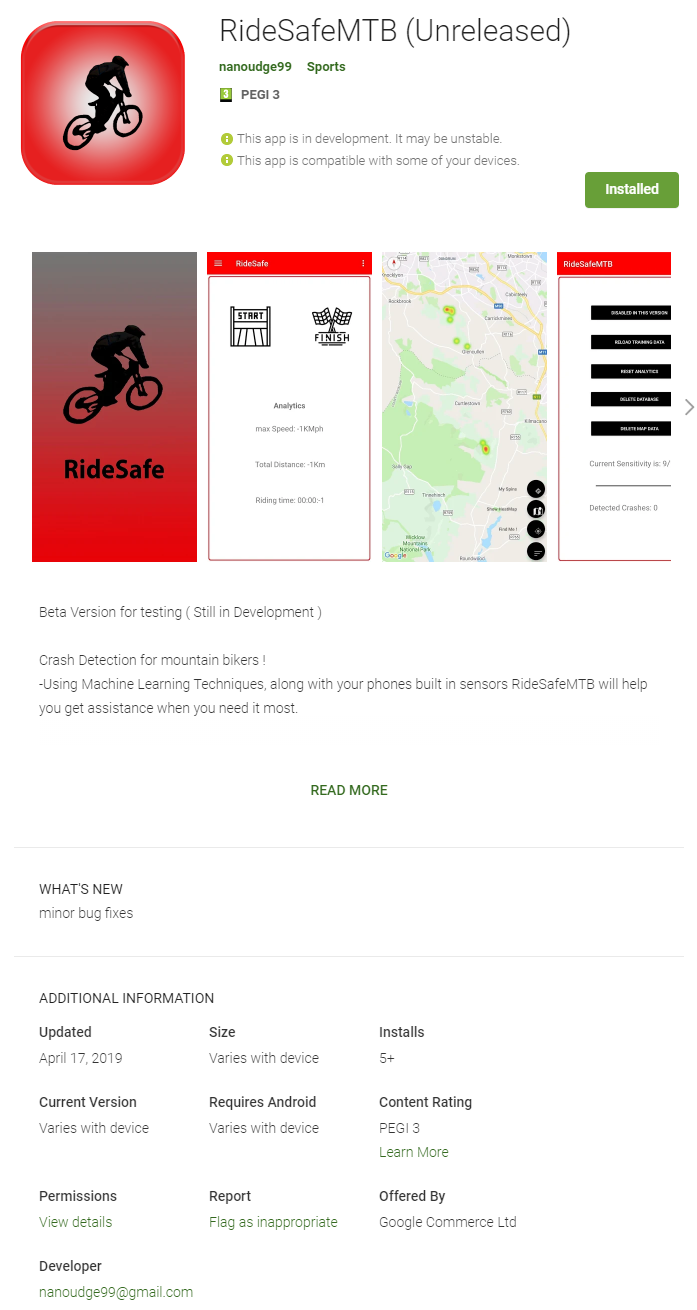
\includegraphics[scale = 1.3]{conclusion/Capture.png}
      \caption{Play Store Listing For RideSafe}
      \label{store}
\end{figure}
%%%%%%%%%%%%%%%%%%%%%%%%%%%%%%%%%%%%%%%%
